% ---------- Titelblad Masterproef Faculteit Wetenschappen -----------
% Dit document is opgesteld voor compilatie met pdflatex.  Indien je
% wilt compileren met latex naar dvi/ps, dien je de figuren naar
% (e)ps-formaat om te zetten.
%                           -- december 2012
% -------------------------------------------------------------------
\RequirePackage{fix-cm}
\documentclass[12pt,a4paper,oneside]{book}

% --------------------- In te laden pakketten -----------------------
% Deze kan je eventueel toevoegen aan de pakketten die je al inlaadt
% als je dit titelblad integreert met de rest van thesis.
% -------------------------------------------------------------------
\usepackage{graphicx,xcolor,textpos}
\usepackage{helvet}
\usepackage{tikz}
\usetikzlibrary{fit,shapes,arrows,positioning,calc}

\usepackage{wrapfig}
\usepackage{chngcntr}
\counterwithout{figure}{chapter}
\counterwithout{table}{chapter}

% -------------------- Pagina-instellingen --------------------------
% Indien je deze wijzigt, zal het titelblad ook wijzigen.  Dit dien je
% dan manueel aan te passen.
% --------------------------------------------------------------------

\topmargin -10mm
\textwidth 160truemm
\textheight 240truemm
\oddsidemargin 0mm
\evensidemargin 0mm

% ------------------- textpos-instellingen ---------------------------
% Enkele andere instellingen voor het voorblad.
% --------------------------------------------------------------------

\definecolor{green}{RGB}{172,196,0}
\definecolor{bluetitle}{RGB}{29,141,176}
\definecolor{blueaff}{RGB}{0,0,128}
\definecolor{blueline}{RGB}{82,189,236}
\setlength{\TPHorizModule}{1mm}
\setlength{\TPVertModule}{1mm}

\renewcommand{\contentsname}{Inhoudstafel}
\renewcommand{\listfigurename}{Lijst van figuren}
\renewcommand{\chaptername}{Hoofdstuk}

\begin{document}

% ---------------------- Voorblad ------------------------------------
% Vergeet niet de tekst aan te passen:
% - Titel en, indien van toepassing, ondertitel
%          voor eventuele formules in de titel of ondertitel
%          gebruik je  \form{$...$}
% - Je naam
% - Je (co)promotor, begeleider (indien van toepassing)
% - Je opleiding
% - Het academiejaar
% --------------------------------------------------------------------
\thispagestyle{empty}
\newcommand{\form}[1]{\scalebox{1.087}{\boldmath{#1}}}
\sffamily
%
\begin{textblock}{191}(-24,-11)
\colorbox{green}{\hspace{113mm}\ \parbox[c][18truemm]{100mm}{\textcolor{white}{FACULTEIT COMPUTERWETENSCHAPPEN}}}
\end{textblock}
%
\begin{textblock}{70}(-18,-19)
\textblockcolour{}
\includegraphics*[height=19.8truemm]{LogoKULeuven}
\end{textblock}
%
\begin{textblock}{160}(-6,63)
\textblockcolour{}
\vspace{-\parskip}
\flushleft
\fontsize{40}{42}\selectfont \textcolor{bluetitle}{Real-Time Cadansaanpassing in een Automatische fietstransmissie }\\[1.5mm]
\end{textblock}
%

\begin{textblock}{160}(8,153)
\textblockcolour{}
\vspace{-\parskip}
\flushright
\fontsize{14}{16}\selectfont \textbf{Arno Cools}
\end{textblock}
%
\begin{textblock}{70}(-6,191)
\textblockcolour{}
\vspace{-\parskip}
\flushleft
Promotor:\\Prof. M. Moens\\[-2pt]
\vspace{5mm}
Begeleider:\\
\textsl{Ir. Tomas Keppens\\Ir. Jorrit Heidbuchel\\Ir. Rugen Heidbuchel}\\[-2pt]
\end{textblock}
%
\begin{textblock}{160}(8,191)
\textblockcolour{}
\vspace{-\parskip}
\flushright
Proefschrift ingediend tot het\\[4.5pt]
behalen van de graad van\\[4.5pt]
Master of Toegepase Informatica\\
\end{textblock}
%
\begin{textblock}{160}(8,232)
\textblockcolour{}
\vspace{-\parskip}
\flushright
Academiejaar 2018-2019
\end{textblock}
%
\begin{textblock}{191}(-24,248)
{\color{blueline}\rule{550pt}{5.5pt}}
\end{textblock}
%
\vfill
\newpage

% Als je het titelblad wil integreren met de rest van je thesis,
% kan je hieronder verder.
% ----------------------- Eerste pagina's -------------------------
% Hier kan je inhoudsopgave, voorwoord en dergelijke kwijt.
% -----------------------------------------------------------------
\rmfamily
\frontmatter
\pagenumbering{roman}
\tableofcontents
\setcounter{page}{0}
\chapter{Voorwoord}

A preface

\chapter{Abstract}

An abstract.

\listoffigures
\addcontentsline{toc}{chapter}{Lijst van figuren}

\chapter{Lijst van symbolen en afkortingen}
lijst van symbolen en afkortingen

\mainmatter
\pagenumbering{arabic}

\chapter{Probleemstelling}
\section{Mobiliteitsvraagstuk}
De auto is het slachtoffer geworden van zijn eigen succes: we staan meer dan ooit in de file en de CO2 van personenverkeer stijgt jaar na jaar. De belg neemt al snel de auto voor korte afstanden ($<$ 25 km). In deze auto zit meestal maar 1 persoon. Het Belgische wagenpark blijft groeien (tabel 1). Hier zien we wel een trend ontstaan. Er worden steeds meer elektrische en hybride wagens verkocht, maar die staan natuurlijk net zo goed in de file. Mobiliteit op twee wielen kan hier een oplossing bieden.
\\
\begin{wrapfigure}{R}{0.45\textwidth}
  \centering
  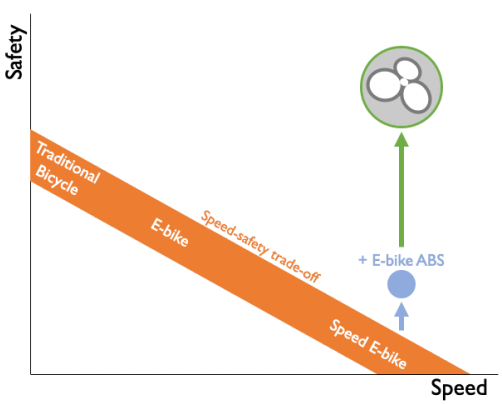
\includegraphics[width=1.1\linewidth]{images/snelheid-veiligheid-tradeoff.png}
  \caption{snelheid-veiligheid trade-off (bron: IntuEdrive)}
  \label{fig:ok}
\end{wrapfigure}

Mobiliteit op twee wielen kennen we al lang: fietsen bestaan al sinds de 19de eeuw. Elektrische fietsen hebben het potentieel van deze tweewielers enorm verhoogd: fietsen wordt moeiteloos en stukken sneller. Spijtig genoeg neemt het risico op ongevallen ook toe bij hogere snelheid. Dat komt omdat e-bikes en speed e-bikes precies dezelfde technologie gebruiken als normale fietsen – grote wielen met smalle banden, kettingaandrijving met manuele versnellingen, mechanische handremmen – bij veel hogere snelheden. IntuEdrive noemt dit de snelheid-veiligheid trade-off. De veiligheid kan beperkt worden verhoogd door componenten toe te voegen (bv. Bosch e-bike ABS), maar de functionaliteit van deze systemen blijft beperkt. Er is een meer holistische aanpak nodig. Bovendien bieden elektrische fietsen vandaag nog niet het gebruiksgemak en de betrouwbaarheid die de consument gewend is van zijn wagen.
\\
IntuEdrive’s CoSaR is een snelle elektrische fiets die veiliger is dan de klassieke mechanische fiets, dankzij hun innovatie tweewielaandrijving en elektrische remfunctie. Dit systeem reduceert de stopafstand met 60\% en maakt schakelen overbodig (automatische versnellingen). Het stapt ook af van de onderhoudsintensieve fietscomponenten (ketting, tandwielen, mechanische remmen). Dit maakt CoSaR de perfecte e-bike voor woon-werkverkeer: makkelijk, veilig en betrouwbaar.
\\
Door automatisch te schakelen zorgt CoSaR ervoor dat de fietser in elke situatie precies zo snel trapt als hij of zij wil. Deze gewenste trapsnelheid – of beter trapcadans – varieert van persoon tot persoon en hangt af van omstandigheden zoals helling, tegenwind en rijsnelheid. Omdat deze gewenste cadans niet op voorhand gekend is, schakelt de transmissie momenteel op basis van een vaste wetmatigheid die tijdens testen getuned is om voor zoveel mogelijk gebruikers comfortabel aan te voelen. Wijkt deze wetmatigheid af van de gewenste cadans van een specifieke gebruiker, dan kan deze gebruiker via knoppen op het stuur tijdens het fietsen zijn of haar cadans manueel aanpassen.
\\
\begin{table}[]
\begin{tabular}{llllll}
 & 2014 & 2015 & 2016 & 2017 & 2018 \\
Personenwagens                              & 5.555.499 & 5.623.579 & 5.712.061 & 5.785.447 & 5.853.782 \\
- rijdend op benzine                        & 2.029.688 & 2.091.327 & 2.199.038 & 2.335.349 & 2.518.942 \\
- rijdend op diesel                         & 3.458.424 & 3.457.526 & 3.424.592 & 3.339.034 & 3.193.658 \\
- rijdend op gas                            & 22.051    & 18.967    & 17.238    & 15.965    & 15.500    \\
- met elektrische motor                     & 1.792     & 2.871     & 4.368     & 6.552     & 9.244     \\
- hybride                                   & 23.444    & 32.151    & 44.364    & 63.740    & 87.012    \\
- niet nader bepaald                        & 20.100    & 20.737    & 22.461    & 24.807    & 29.426    \\
Inwoners per personenauto  & 2,01      & 1,99      & 1,97      & 1,96      & 1,94     
\end{tabular}
 \caption{Grootte van het voertuigenpark 2014-2018 (bron: statbel.fgov.be)} 	\label{table:Grootte van het voertuigenpark 2014-2018}
\end{table}	
\section{Online machine learning voor geïndividualiseerde cadanscontrole}

 
\chapter{Methode}
\chapter{Resultaten}
\chapter{Discussie}

\tikzset{
block/.style = {draw, fill=white, rectangle, minimum height=3em, minimum width=9em},
tmp/.style  = {coordinate}, 
input/.style = {coordinate},
output/.style= {coordinate},
box/.style={draw=gray,dashed,fill opacity = 0,thick,inner sep=5pt},
test/.style = {}
}
\begin{figure}
\begin{tikzpicture}[auto, node distance=2cm,>=latex']
    \node [input, name=fietsinput] (fietsinput) {};
    \node [block, right of=fietsinput,node distance=5cm] (fietser) {Fietser};
    \node [tmp, right of=fietser,node distance=3cm] (above_fietser){};
    \node [block, below of=above_fietser,node distance=3cm] (fiets) {Fiets};
    \node [tmp, left = 1.5cm of fiets] (left_fiets) {};
    \node [block, below of=fiets] (controller){Controller};
    \node [tmp, left = 1.5cm of controller] (left_controller) {};
    \node [block, below of=controller] (cadencecontroller) {Cadanscontroller};   
    \node [tmp, left = 1.5cm of cadencecontroller] (left_cadencecontrol) {};
    \node [tmp, right of=fiets,node distance=3cm] (right_fiets){};    
    \node [tmp, right of=right_fiets] (output){};    
    \draw [->] (fietsinput) -- node{$r$} (fietser);
    \draw [->] (fietser) |- (above_fietser) -- node{$u_{cy}$} (fiets);
    \draw [->] (controller.west) |- (left_controller) |- node {$u_{contr}$} (fiets.west);
    \draw [->] (cadencecontroller) -- node{$FCC_{est}$} (controller);
   	\draw [->] (right_fiets) |- (controller.east);
   	\draw [->] (right_fiets) |- (cadencecontroller.east);
    \draw [->] (fiets) -- node [name=y] {$y$}(output);   
\end{tikzpicture}
\caption{Blokdiagram van het fiets-fietser-controller systeem}
  \label{fig:Blokdiagram van het fiets-fietser-controller systeem}
\end{figure}



\newpage
% ----------------------- Achterblad ------------------------------
% Vergeet niet de tekst aan te passen:
% - Afdeling
% - Adres van de afdeling
% - Telefoon en faxnummer
% -----------------------------------------------------------------
\thispagestyle{empty}
\sffamily
%
\begin{textblock}{191}(113,-11)
{\color{blueline}\rule{160pt}{5.5pt}}
\end{textblock}
%
\begin{textblock}{191}(168,-11)
{\color{blueline}\rule{5.5pt}{59pt}}
\end{textblock}
%
\begin{textblock}{183}(-24,-11)
\textblockcolour{}
\flushright
\fontsize{7}{7.5}\selectfont
\textbf{Computerwetenschappen}\\
Celestijnenlaan 200 A bus 2402\\
3000 LEUVEN, BELGI\"{E}\\
tel. + 32 16 32 77 00\\
fax + 32 16 32 79 96\\
www.kuleuven.be\\
\end{textblock}
%
\begin{textblock}{191}(154,-7)
\textblockcolour{}
\includegraphics*[height=16.5truemm]{sedes}
\end{textblock}
%
\begin{textblock}{191}(-20,235)
{\color{bluetitle}\rule{544pt}{55pt}}
\end{textblock}
\end{document}
